%%%%%%%%%%%%%%%%%%%%%%%%%%%%%%%%%%%%%%%%%%%%%%%%%%%%%%%%%%%%%%%%%%%%%%%%%%
%%%%%%%%%%%%%%%%%%%%%%%%%%%%%%%%%%%%%%%%%%%%%%%%%%%%%%%%%%%%%%%%%%%%%%%%%%
\clearpage{}
\section{WW$\gamma$/WZ$\gamma$ cross section measurement}
\label{sec:sys}
% ---- ---- ---- ---- ---- ---- ---- ---- ---- ---- ---- ---- ---- ---- ----
%A measurement of the WW$\gamma$/WZ$\gamma$ cross section is derived using
%
%\begin{center}
%\begin{equation}
%   \sigma = \frac{N_{data}-N_{bkg}}{L \cdot A \cdot \varepsilon_{MC} \cdot SF}
%\label{eq:xsection}
%\end{equation}
%\end{center}
%
%where $\sigma$ is the measured cross section, $N_{data}$ is the number of
%selected events observed in data, $N_{bkg}$ is the number of selected 
%background events predicted from Monte Carlo, L is the integrated 
%luminosity, A is the signal acceptance predicted from Monte Carlo, 
%$\varepsilon_{MC}$ is the Monte Carlo event selection efficiency, and SF 
%is the efficiency scale factor between data and Monte Carlo 
%($\frac{\varepsilon_{data}}{\varepsilon_{MC}}$), such as those listed for
%the photon in Table~\ref{tab:photon_eff}.  Each of these values has an 
%associated systematic and statistical error that must be propagated 
%through equation~\ref{eq:xsection}.  Using standard error propagation, 
%the uncertainty in the cross sectional measurement is derived using
%
%\begin{center}
%\begin{equation}
%  \delta\sigma = |\sigma|\sqrt{(\frac{{\delta}N_{sig}}{N_{sig}})^{2}+(\frac{{\delta}L}{L})^{2}+(\frac{{\delta}A}{A})^{2}+(\frac{\delta\varepsilon_{MC}}{\varepsilon_{MC}})^{2}+(\frac{{\delta}SF}{SF})^{2}}
%\label{eq:xsec_unc}
%\end{equation}
%\end{center}

%where $N_{sig}$ = $N_{data}-N_{bkg}$ and thus

%\begin{center}
%\begin{equation}
%   {\delta}N_{sig} = \sqrt{({\delta}N_{data})^{2}+({\delta}N_{bkg})^{2}}.
%\end{equation}
%\end{center}

%With equations~\ref{eq:xsection} and \ref{eq:xsec_unc}, Table~\ref{tab:xsec_num} lists the values used to measure the WW$\gamma$ cross section.

%\begin{table}[htb]
%\centering
%\scalebox{0.70}{
%  \begin{tabular}{|c|c|c|c|}
%  \hline
%  Variable & Value & Systematic Uncertainty & Statistical Uncertainty \\
%  \hline
%  \hline
%  $N_{data}$                          & 98.0 & ----   & 9.9   \\
%  $N_{bkg}$                           & 112.6 & 9.7   & 4.7   \\
%  L                                   & 19.3  & ----   & 0.6    \\
%  A $\cdot \varepsilon_{MC} \cdot$ SF & 0.004 & 0.0002 & 0.0002 \\
%  \hline
%  \end{tabular}}
%  \caption{List of values and uncertainties used in measuring the WW$\gamma$ cross section.}
%  \label{tab:xsec_num}
%\end{table}

%Using the values in Table~\ref{tab:xsec_num}, the measured cross section for WW$\gamma$ is $\sigma$ = -168.4 $\pm$ 112.9 (Sys.) $\pm$ 127.0 (Stat.) fb.  This measurement takes into account the K-factors used for WW$\gamma$/WZ$\gamma$ and W$\gamma$+Jets processes listed in Section~\ref{sec:Kfact}, as well as the MVA discussed in Section~\ref{sec:MVA}.  The theoretical cross section provided by MadGraph 5 for semileptonic WW$\gamma$ is 41 fb, again taking into account the K-factor for WW$\gamma$ listed in Section~\ref{sec:Kfact}~\cite{MadGraph}.

This SM cross sectional measurement's uncertainties are large due to the low signal 
statistics, the uncertainties in the K-factors used, and the fake photon 
rate's systematic uncertainty of 12-39\%; therefore, we cannot claim an 
observation of WW$\gamma$ events.

The Standard Model WW$\gamma$/WZ$\gamma$ signal strength with and without
MVA optimization is shown in Figure~\ref{fig:signalstrength}, with the 
1-$\sigma$ and 2-$\sigma$ bands. Figure~\ref{fig:signalstrength} 
demonstrates that a signal strength below 1 suggests we are sensitive to 
the signal and can measure the cross section; however, we are well above 
a value of 1 and are therefore not sensitive to the SM signal. It can be 
seen that MVA optimization makes a small improvement on our sensitivity,
and optimizes our sensitivity at a MVA cut of 0.2. 
While the MVA selection helps to improve sensitivity of the measurement it is not changing the fact that only a upper cross section limit is derived for $WV\gamma$. 
Thus we consider the $WV\gamma$ upper cross section limit without use of MVA as the primary result and keep the study documented for future iterations of the analysis.

\begin{figure}[h]
  \begin{center}
    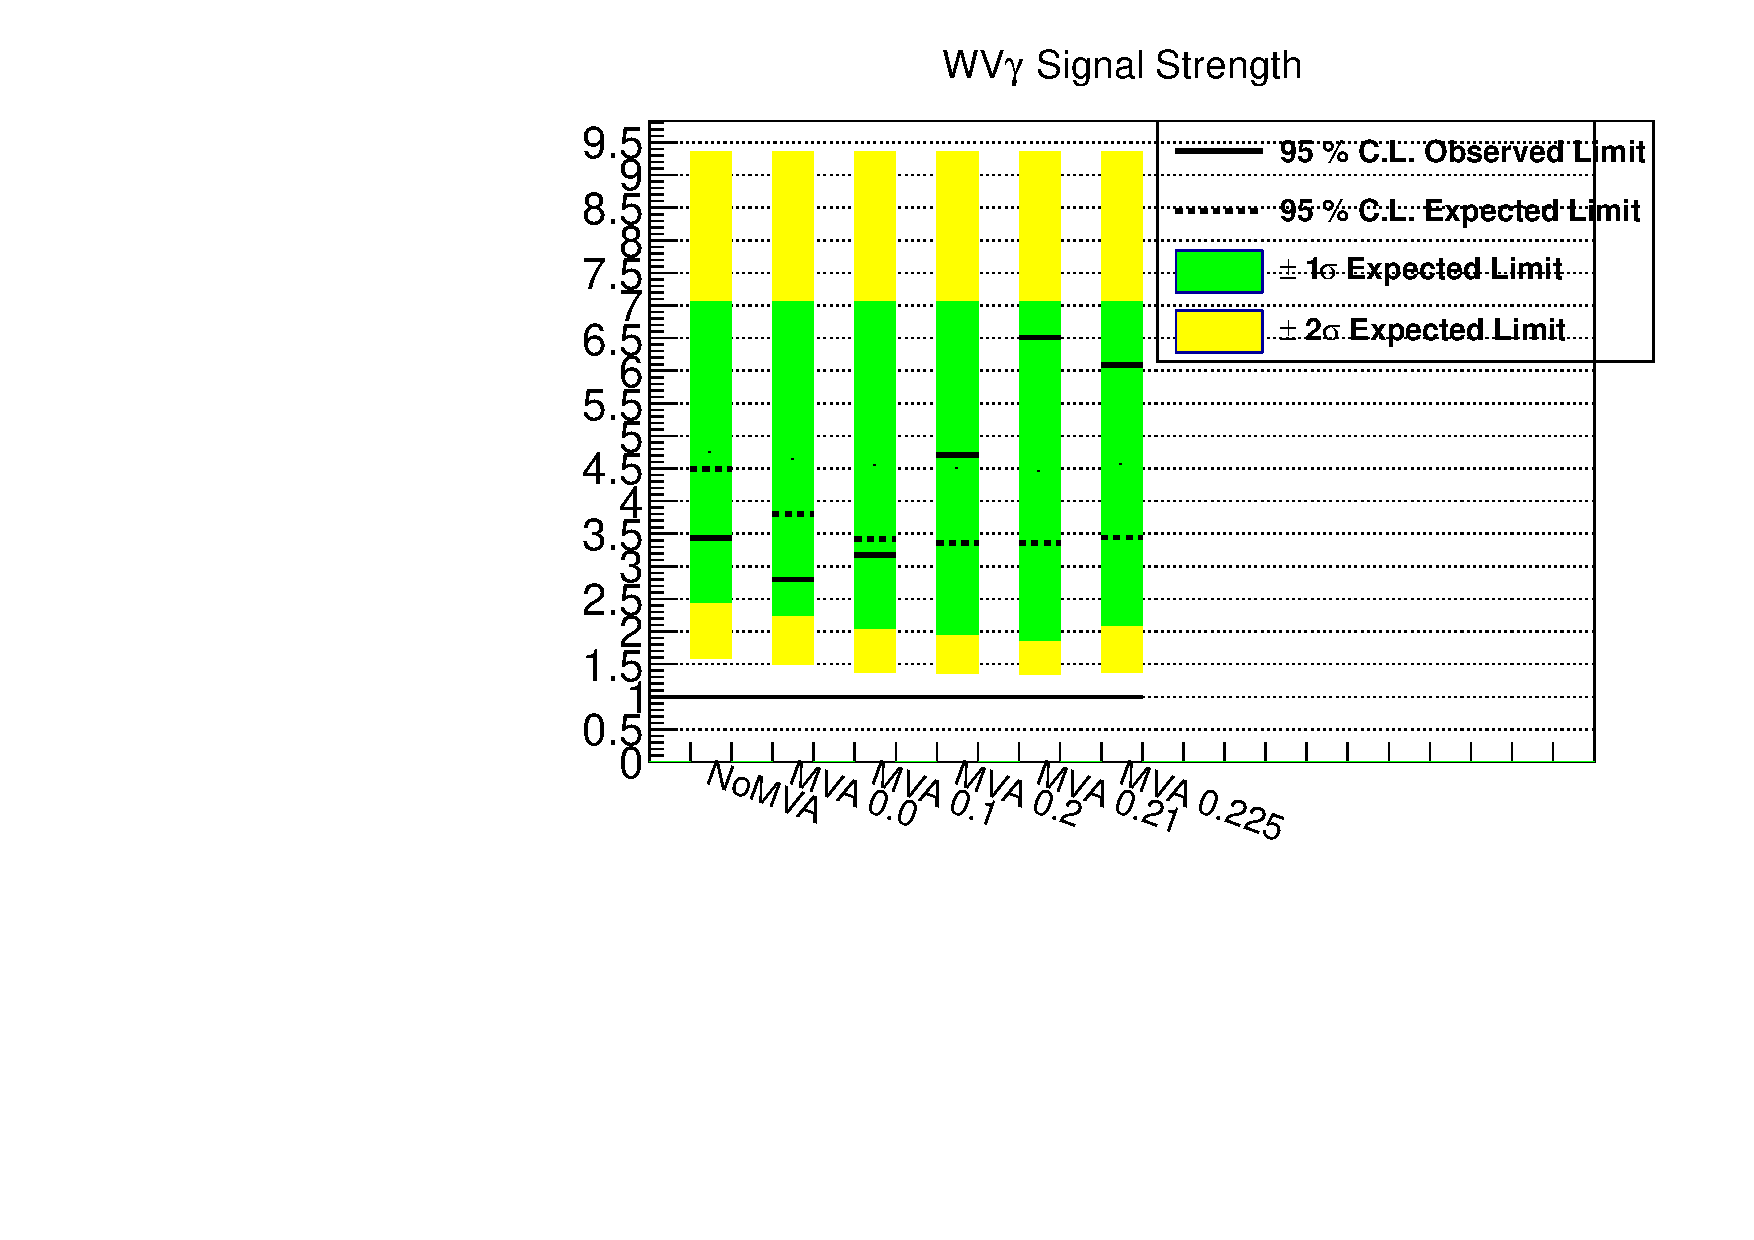
\includegraphics[width=0.75\textwidth]{figs/WVAsignalstrength.pdf}
    \caption{Standard Model WW$\gamma$/WZ$\gamma$ signal strength with various MVA cut values. A strength at or below 1 suggests we are sensitive to the SM signal.}
    \label{fig:signalstrength}
  \end{center}
\end{figure}


